\let\negmedspace\undefined
\let\negthickspace\undefined
\documentclass[journal]{IEEEtran}
\usepackage[a5paper, margin=10mm, onecolumn]{geometry}
%\usepackage{lmodern} % Ensure lmodern is loaded for pdflatex
\usepackage{tfrupee} % Include tfrupee package

\setlength{\headheight}{1cm} % Set the height of the header box
\setlength{\headsep}{0mm}     % Set the distance between the header box and the top of the text

\usepackage{gvv-book}
\usepackage{gvv}
\usepackage{cite}
\usepackage{amsmath,amssymb,amsfonts,amsthm}
\usepackage{algorithmic}
\usepackage{graphicx}
\usepackage{textcomp}
\usepackage{xcolor}
\usepackage{txfonts}
\usepackage{listings}
\usepackage{enumitem}
\usepackage{mathtools}
\usepackage{gensymb}
\usepackage{comment}
\usepackage[breaklinks=true]{hyperref}
\usepackage{tkz-euclide} 
\usepackage{listings}
% \usepackage{gvv}                                        
\def\inputGnumericTable{}                                 
\usepackage[latin1]{inputenc}                                
\usepackage{color}                                            
\usepackage{array}                                            
\usepackage{longtable}                                       
\usepackage{calc}                                             
\usepackage{multirow}                                         
\usepackage{hhline}                                           
\usepackage{ifthen}                                           
\usepackage{lscape}
\begin{document}

\bibliographystyle{IEEEtran}
\vspace{3cm}

\title{9.2.5}
\author{EE24BTECH11016 - DHWANITH M DODDAHUNDI}
% \maketitle
% \newpage
% \bigskip
{\let\newpage\relax\maketitle}

\renewcommand{\thefigure}{\theenumi}
\renewcommand{\thetable}{\theenumi}
\setlength{\intextsep}{10pt} % Space between text and floats


\numberwithin{equation}{enumi}
\numberwithin{figure}{enumi}
\renewcommand{\thetable}{\theenumi}


			\textbf{QUESTION}:\\
Consider the differential equation $xy^{\prime}=y (x\neq0)$ . Verify that $y = Ax$ is a solution for it, given the initial conditions $ y \brak{1} = A $ . \\
\textbf{SOLUTION}: \\
%\begin{tabular}[12pt]{ |c| c| c |}
    \hline
    \textbf{Variable} & \textbf{Description} & \textbf{values}\\ 
    \hline
    $\vec{V}$ & Quadratic form of the matrix & $\myvec{1 & 0 \\ 0 & 1} $\\
    \hline
    $\vec{u}$ & Linear coefficient vector & $\myvec{0 \\ 0} $\\
    \hline
    f & constant term & -4 \\ 
    \hline
    $\vec{m}$ & The direction vector of line & $\myvec{1 \\ 0}$\\
    \hline
     $\vec{h}$ & Point on line & \myvec{2 \\ 0} \\
     \hline
\end{tabular}
 \\ \\ \\
Consider the differential equation, 
\begin{align} 
	 xy^{\prime}=y (x\neq0)\label{eq:third} 
\end{align}
\begin{align}
    y^{\prime}=\frac{y}{x}\label{eq:fourth} 
\end{align}
\begin{align}
    \frac{dy}{dx}=\frac{y}{x}
\end{align}
Since the Laplace transform works best with initial conditions defined at $x=0$, we change the variable by letting:
\begin{align}
    t=\log{(x)},x=e^{t}.
\end{align}
\begin{align}
    \frac{d}{dx}=\frac{d}{dt}\cdot\frac{dt}{dx}=\frac{d}{dx}\cdot\frac{1}{x}
\end{align}
Thus, the equation becomes:
\begin{align}
	\frac{dy}{dt}\cdot\frac{1}{x}=\frac{y}{x} \\
    \frac{dy}{dt}=y
\end{align}
Taking the Laplace transform of both sides:
\begin{align}
	\mathcal{L} \brak{\frac{dy}{dt}}= \mathcal{L} \brak{y} \\
    sY\brak{s}-y\brak{0}=Y\brak{s}
\end{align}
Rearranging,
\begin{align}
	\brak{s-1}Y\brak{s}=y\brak{0} \\
    Y\brak{s}=\frac{y\brak{0}}{s-1}
\end{align} 
\newpage
From the original problem, $y\brak{1}=A$. Substituting $x=1$ (or $t=\log{\brak{1}}=0$), we find $y\brak{0}=A$. So:
\begin{align}
	 Y\brak{s}=\frac{A}{s-1} \\
  \mathcal{L} \brak{y\brak{t}} = \frac{A}{s-1}    
\end{align}
Now, take the inverse laplace transform 
\begin{align}
  y\brak{t}=\mathcal{L}^{-1} \brak{\frac{A}{s-1}} \\
    y\brak{t}=A\cdot \mathcal{L}^{-1} \brak{\frac{1}{s-1}} \\
    y\brak{t}=A\cdot e^{t}
\end{align}
Returning to the original variable $x=e^{t}$, we get:
\begin{align}
    y\brak{x}=A\cdot e^{\ln{x}}=Ax
\end{align}
Hence, verified. \\
\newline 
\textbf{ALGORITHM :} \\
\begin{align}
	 x_0 &= 1 \\
	 y_0 &= 1 \text{(when $A=1$)}   \\
	 h &= 0.01 \\
	 x_{n+1} &= x_{n} + h \\
	 y_{n+1} &= y_{n} + h \brak{y^{\prime}} 
\end{align}
From \eqref{eq:fourth}, 
\begin{align}
	y_{n+1} = y_{n} + h \brak{\frac{y_{n}}{x_{n}}} \\
	y_{n+1} = y_{n} + h \brak{1}
\end{align}
which is the required difference equation.

\begin{figure}[h]
				 \centering
				 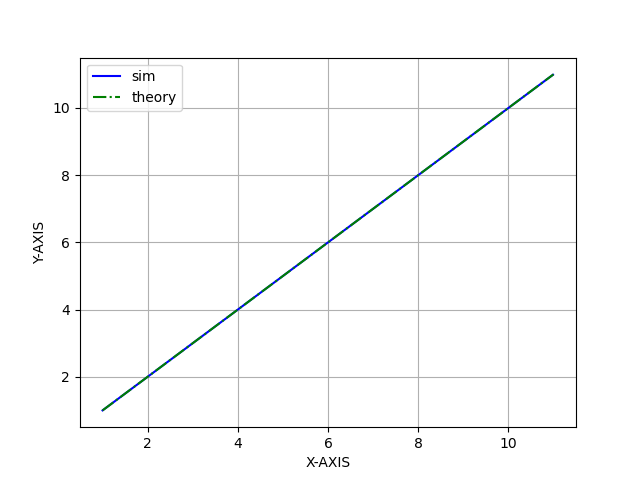
\includegraphics[width=\columnwidth]{figs/fig.png}
				 \caption{A plot of the given question.}
				 \label{fig:Plot1}
			 \end{figure}


\end{document}
